\subsection{Microcontroller}
\schematicpage{13}{MPU}

To provide control, communications, and on-board data processing, the
instrument contains a microcontroller. This is an Atmel deviced based
on the ARM Cortex-M4 core, with 256~kiB of flash memory, 64~kiB of RAM,
a 120~MHz maximum clock speed, and USB connectivity. The microcontroller
is provided with a separately regulated 3.3~V rail, and has an internal
regulator to supply a separate, internal 1.2~V rail for itself. It is
connected to a standard ARM JTAG port on the PCB to allow programming and
debug, and connects directly to a PC via USB, to the synthesizer IC via
SPI (Serial Peripheral Interface), to other miscellaneous subcircuits via
GPIO (General Purpose Input/Output), and to the logarithmic amplifier using
its on-chip ADC (Analog to Digital Converter).

\subsubsection{USB Communications}
\schematicpage{2}{Comm}
\begin{framed}
Also relevant: \hyperref[ssc:usbpower]{USB Power Input Circuit}
\end{framed}

A simple conditioning circuit is placed between the USB power and
the microcontroller:

\begin{figure}[H]
\centering
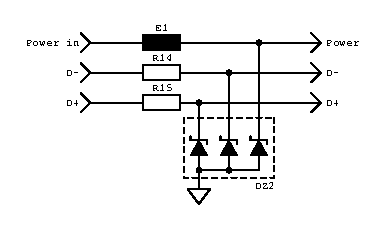
\includegraphics{too/usbprot}
\caption{USB conditioning circuit}
\label{fig:usbcond}
\end{figure}

\refdes{E1} is a ferrite bead, which absorbs RF noise and dissipates it as heat.
\refdes{R14} and \refdes{R15} increase the impedance of the USB lines, bringing
them closer to the correct value (as the microcontroller's USB output impedance
is too load). \refdes{DZ2} is a triple ESD-protection Zener diode package, which
clamps and dissipates pulses of static charge that might be applied to the port,
and prevents them from reaching downstream circuitry.
